\documentclass[fontsize=11pt,
titlepage=true,
footnotes=multiple
]{scrartcl}

%headers
\usepackage{scrlayer-scrpage}

%define colors
\usepackage[dvipsnames]{xcolor}
\definecolor{twriblue}{RGB}{0, 84, 164}

%fonts, lmodern is the fallback if system fonts arent installed
%\usepackage{lmodern}
\usepackage{amssymb,amsmath}
\usepackage{ifxetex,ifluatex}
\usepackage{fixltx2e} % provides \textsubscript
\ifxetex
  \usepackage{mathspec}
  \usepackage{xltxtra,xunicode}
\else
  \usepackage{fontspec}
\defaultfontfeatures{Ligatures=TeX,Scale=MatchLowercase}
\newcommand{\euro}{€}

\setmainfont{Minion Pro-Regular}[BoldFont={Minion Pro-Bold},
ItalicFont={Minion Pro-It},
BoldItalicFont={Minion Pro MediumIt}]

\setsansfont{Open Sans-Regular}[BoldFont={OpenSans-Bold},
ItalicFont={OpenSans-Italic},
BoldItalicFont={OpenSans-BoldItalic}]


% % %\fi

\addtokomafont{section}{\textcolor{twriblue}}
\addtokomafont{subsection}{\textcolor{twriblue}}

% use upquote if available, for straight quotes in verbatim environments
\IfFileExists{upquote.sty}{\usepackage{upquote}}{}
% use microtype if available
\IfFileExists{microtype.sty}{%
\usepackage{microtype}
\UseMicrotypeSet[protrusion]{basicmath} % disable protrusion for tt fonts
}{}
\usepackage{color}
\usepackage{fancyvrb}
\newcommand{\VerbBar}{|}
\newcommand{\VERB}{\Verb[commandchars=\\\{\}]}
\DefineVerbatimEnvironment{Highlighting}{Verbatim}{commandchars=\\\{\}}
% Add ',fontsize=\small' for more characters per line
\usepackage{framed}
\definecolor{shadecolor}{RGB}{248,248,248}
\newenvironment{Shaded}{\begin{snugshade}}{\end{snugshade}}
\newcommand{\AlertTok}[1]{\textcolor[rgb]{0.94,0.16,0.16}{#1}}
\newcommand{\AnnotationTok}[1]{\textcolor[rgb]{0.56,0.35,0.01}{\textbf{\textit{#1}}}}
\newcommand{\AttributeTok}[1]{\textcolor[rgb]{0.77,0.63,0.00}{#1}}
\newcommand{\BaseNTok}[1]{\textcolor[rgb]{0.00,0.00,0.81}{#1}}
\newcommand{\BuiltInTok}[1]{#1}
\newcommand{\CharTok}[1]{\textcolor[rgb]{0.31,0.60,0.02}{#1}}
\newcommand{\CommentTok}[1]{\textcolor[rgb]{0.56,0.35,0.01}{\textit{#1}}}
\newcommand{\CommentVarTok}[1]{\textcolor[rgb]{0.56,0.35,0.01}{\textbf{\textit{#1}}}}
\newcommand{\ConstantTok}[1]{\textcolor[rgb]{0.00,0.00,0.00}{#1}}
\newcommand{\ControlFlowTok}[1]{\textcolor[rgb]{0.13,0.29,0.53}{\textbf{#1}}}
\newcommand{\DataTypeTok}[1]{\textcolor[rgb]{0.13,0.29,0.53}{#1}}
\newcommand{\DecValTok}[1]{\textcolor[rgb]{0.00,0.00,0.81}{#1}}
\newcommand{\DocumentationTok}[1]{\textcolor[rgb]{0.56,0.35,0.01}{\textbf{\textit{#1}}}}
\newcommand{\ErrorTok}[1]{\textcolor[rgb]{0.64,0.00,0.00}{\textbf{#1}}}
\newcommand{\ExtensionTok}[1]{#1}
\newcommand{\FloatTok}[1]{\textcolor[rgb]{0.00,0.00,0.81}{#1}}
\newcommand{\FunctionTok}[1]{\textcolor[rgb]{0.00,0.00,0.00}{#1}}
\newcommand{\ImportTok}[1]{#1}
\newcommand{\InformationTok}[1]{\textcolor[rgb]{0.56,0.35,0.01}{\textbf{\textit{#1}}}}
\newcommand{\KeywordTok}[1]{\textcolor[rgb]{0.13,0.29,0.53}{\textbf{#1}}}
\newcommand{\NormalTok}[1]{#1}
\newcommand{\OperatorTok}[1]{\textcolor[rgb]{0.81,0.36,0.00}{\textbf{#1}}}
\newcommand{\OtherTok}[1]{\textcolor[rgb]{0.56,0.35,0.01}{#1}}
\newcommand{\PreprocessorTok}[1]{\textcolor[rgb]{0.56,0.35,0.01}{\textit{#1}}}
\newcommand{\RegionMarkerTok}[1]{#1}
\newcommand{\SpecialCharTok}[1]{\textcolor[rgb]{0.00,0.00,0.00}{#1}}
\newcommand{\SpecialStringTok}[1]{\textcolor[rgb]{0.31,0.60,0.02}{#1}}
\newcommand{\StringTok}[1]{\textcolor[rgb]{0.31,0.60,0.02}{#1}}
\newcommand{\VariableTok}[1]{\textcolor[rgb]{0.00,0.00,0.00}{#1}}
\newcommand{\VerbatimStringTok}[1]{\textcolor[rgb]{0.31,0.60,0.02}{#1}}
\newcommand{\WarningTok}[1]{\textcolor[rgb]{0.56,0.35,0.01}{\textbf{\textit{#1}}}}
\usepackage{longtable,booktabs}
\usepackage{graphicx}
\makeatletter
\def\maxwidth{\ifdim\Gin@nat@width>\linewidth\linewidth\else\Gin@nat@width\fi}
\def\maxheight{\ifdim\Gin@nat@height>\textheight\textheight\else\Gin@nat@height\fi}
\makeatother
% Scale images if necessary, so that they will not overflow the page
% margins by default, and it is still possible to overwrite the defaults
% using explicit options in \includegraphics[width, height, ...]{}
\setkeys{Gin}{width=\maxwidth,height=\maxheight,keepaspectratio}
\ifxetex
  \usepackage[setpagesize=false, % page size defined by xetex
              unicode=false, % unicode breaks when used with xetex
              xetex]{hyperref}
\else
  \usepackage[unicode=true]{hyperref}
\fi
\hypersetup{breaklinks=true,
            bookmarks=true,
            pdfauthor={},
            pdftitle={Report Title},
            colorlinks=true,
            citecolor=twriblue,
            urlcolor=twriblue,
            linkcolor=black,
            pdfborder={0 0 0}}
\urlstyle{same}  % don't use monospace font for urls
\setlength{\parindent}{0pt}
\setlength{\parskip}{6pt plus 2pt minus 1pt}
\setlength{\emergencystretch}{3em}  % prevent overfull lines
\setcounter{secnumdepth}{5}

%%% Use protect on footnotes to avoid problems with footnotes in titles
\let\rmarkdownfootnote\footnote%
\def\footnote{\protect\rmarkdownfootnote}


% packages used by kableExtra
\usepackage{pdflscape}
\usepackage{threeparttable}
\usepackage{threeparttablex}
\usepackage{float}
\usepackage{makecell}
% Caption justification
\usepackage{caption}
\captionsetup{justification=raggedright,singlelinecheck=false}
% Box shading
\usepackage{framed,color}
\definecolor{shadecolor}{RGB}{248,248,248}

\makeatletter
\let\@fnsymbol\@arabic %footnote numbers in title page not symbols
\newenvironment{kframe}{%
\medskip{}
\setlength{\fboxsep}{.8em}
 \def\at@end@of@kframe{}%
 \ifinner\ifhmode%
  \def\at@end@of@kframe{\end{minipage}}%
  \begin{minipage}{\columnwidth}%
 \fi\fi%
 \def\FrameCommand##1{\hskip\@totalleftmargin \hskip-\fboxsep
 \colorbox{shadecolor}{##1}\hskip-\fboxsep
     % There is no \\@totalrightmargin, so:
     \hskip-\linewidth \hskip-\@totalleftmargin \hskip\columnwidth}%
 \MakeFramed {\advance\hsize-\width
   \@totalleftmargin\z@ \linewidth\hsize
   \@setminipage}}%
 {\par\unskip\endMakeFramed%
 \at@end@of@kframe}
\makeatother

\renewenvironment{Shaded}{\begin{kframe}}{\end{kframe}}

%format equation cross references
\usepackage{cleveref}

\renewcommand{\eqref}{\Cref}
\Crefformat{equation}{#2#1#3}

% allow landscape and portrait layouts
\usepackage{lscape}
\newcommand{\blandscape}{\begin{landscape}}
\newcommand{\elandscape}{\end{landscape}}


\newlength{\cslhangindent}
\setlength{\cslhangindent}{1.5em}
% For Pandoc 2.8 to 2.11
\newenvironment{cslreferences}%
  {}%
  {\par}
% For pandoc 2.11+ using new --citeproc
\newlength{\csllabelwidth}
\setlength{\csllabelwidth}{3em}
\newenvironment{CSLReferences}[3] % #1 hanging-ident, #2 entry spacing
 {% don't indent paragraphs
  \setlength{\parindent}{0pt}
  % turn on hanging indent if param 1 is 1
  \ifodd #1 \everypar{\setlength{\hangindent}{\cslhangindent}}\ignorespaces\fi
  % set entry spacing
  \ifnum #2 > 0
  \setlength{\parskip}{#2\baselineskip}
  \fi
 }%
 {}
\usepackage{calc}
\newcommand{\CSLBlock}[1]{#1\hfill\break}
\newcommand{\CSLLeftMargin}[1]{\parbox[t]{\csllabelwidth}{#1}}
\newcommand{\CSLRightInline}[1]{\parbox[t]{\linewidth - \csllabelwidth}{#1}}
\newcommand{\CSLIndent}[1]{\hspace{\cslhangindent}#1}

\begin{document}

\begin{titlepage}

% % \thispagestyle{scrheadings}
% \cfoot{
\includegraphics[height=.75in]{logo.png}}
% \thispagestyle{scrheadings}
% 
\vspace*{4\baselineskip}
\begin{center}
\sffamily{\Huge\textcolor{twriblue}{Report Title}}


\rmfamily\normalsize{April 1, 2021}


\rmfamily\normalsize{John Doe\footnote{Texas Water Resources Institute\label{twri}} \footnote{Texas A\&M AgriLife Research\label{agr}}\\
Jane Doe\footnote{Texas A\&M AgriLife Extension Service\label{ext}}\\
Jack Doe\footref{twri}}


\rmfamily\normalsize{Texas Water Resources Institute\\
College Station, TX\\
TR-9999}
\mbox{}
\vfill
\rmfamily\normalsize{Insert other funding or partnership acknowledgments here. Delete this line if it isn't required.}
\vspace{10mm} %10mm vertical space


\includegraphics[height=.75in]{logo.png}

\end{center}
\end{titlepage}
{
\hypersetup{linkcolor=black}
\setcounter{tocdepth}{2}
\tableofcontents
}
\listoftables
\listoffigures


\lohead*{Report Title}

\section*{List of Acronyms}

\begin{longtable}[]{@{}ll@{}}
\toprule
Acronym & Long Name \\
\midrule
\endhead
\emph{E. coli} & \emph{Escherichia coli} \\
FDC & Flow Duration Curve \\
TWRI & Texas Water Resources Institute \\
\bottomrule
\end{longtable}

\newpage

\hypertarget{executive-summary}{%
\section*{Executive Summary}\label{executive-summary}}
\addcontentsline{toc}{section}{Executive Summary}

We might include an executive summary or abstract here.

\newpage

\hypertarget{headings}{%
\section{Headings}\label{headings}}

Main document text starts here!

\hypertarget{second-level-heading}{%
\subsection{Second Level Heading}\label{second-level-heading}}

\hypertarget{third-level-heading}{%
\subsubsection{Third Level Heading}\label{third-level-heading}}

First, second, and third level headings are defined by \texttt{\#}, \texttt{\#\#}, and \texttt{\#\#\#} respectively.

\hypertarget{unumbered-heading}{%
\section*{Unumbered heading}\label{unumbered-heading}}
\addcontentsline{toc}{section}{Unumbered heading}

Headings are automatically numbered. If you want a section heading to remain unnumbered use \texttt{\{-\}} after the heading.

\hypertarget{tables}{%
\section{Tables}\label{tables}}

Raw data output will not format as a table. Use \texttt{knitr::kable()} or the \href{https://haozhu233.github.io/kableExtra/}{\texttt{kableExtra}} package to format tables.
This is an example of how we cross-reference that table (Table \ref{tab:mtcars}).

\begin{table}

\caption{\label{tab:mtcars}this is the builtin mtcars data.}
\centering
\begin{tabular}[t]{lrrrrrrrrrrr}
\toprule
  & mpg & cyl & disp & hp & drat & wt & qsec & vs & am & gear & carb\\
\midrule
Mazda RX4 & 21.0 & 6 & 160.0 & 110 & 3.90 & 2.620 & 16.46 & 0 & 1 & 4 & 4\\
Mazda RX4 Wag & 21.0 & 6 & 160.0 & 110 & 3.90 & 2.875 & 17.02 & 0 & 1 & 4 & 4\\
Datsun 710 & 22.8 & 4 & 108.0 & 93 & 3.85 & 2.320 & 18.61 & 1 & 1 & 4 & 1\\
Hornet 4 Drive & 21.4 & 6 & 258.0 & 110 & 3.08 & 3.215 & 19.44 & 1 & 0 & 3 & 1\\
Hornet Sportabout & 18.7 & 8 & 360.0 & 175 & 3.15 & 3.440 & 17.02 & 0 & 0 & 3 & 2\\
\addlinespace
Valiant & 18.1 & 6 & 225.0 & 105 & 2.76 & 3.460 & 20.22 & 1 & 0 & 3 & 1\\
Duster 360 & 14.3 & 8 & 360.0 & 245 & 3.21 & 3.570 & 15.84 & 0 & 0 & 3 & 4\\
Merc 240D & 24.4 & 4 & 146.7 & 62 & 3.69 & 3.190 & 20.00 & 1 & 0 & 4 & 2\\
Merc 230 & 22.8 & 4 & 140.8 & 95 & 3.92 & 3.150 & 22.90 & 1 & 0 & 4 & 2\\
Merc 280 & 19.2 & 6 & 167.6 & 123 & 3.92 & 3.440 & 18.30 & 1 & 0 & 4 & 4\\
\bottomrule
\end{tabular}
\end{table}

\hypertarget{figures}{%
\section{Figures}\label{figures}}

We can embed and cross-reference plots (Figure \ref{fig:pressure}).

\begin{figure}
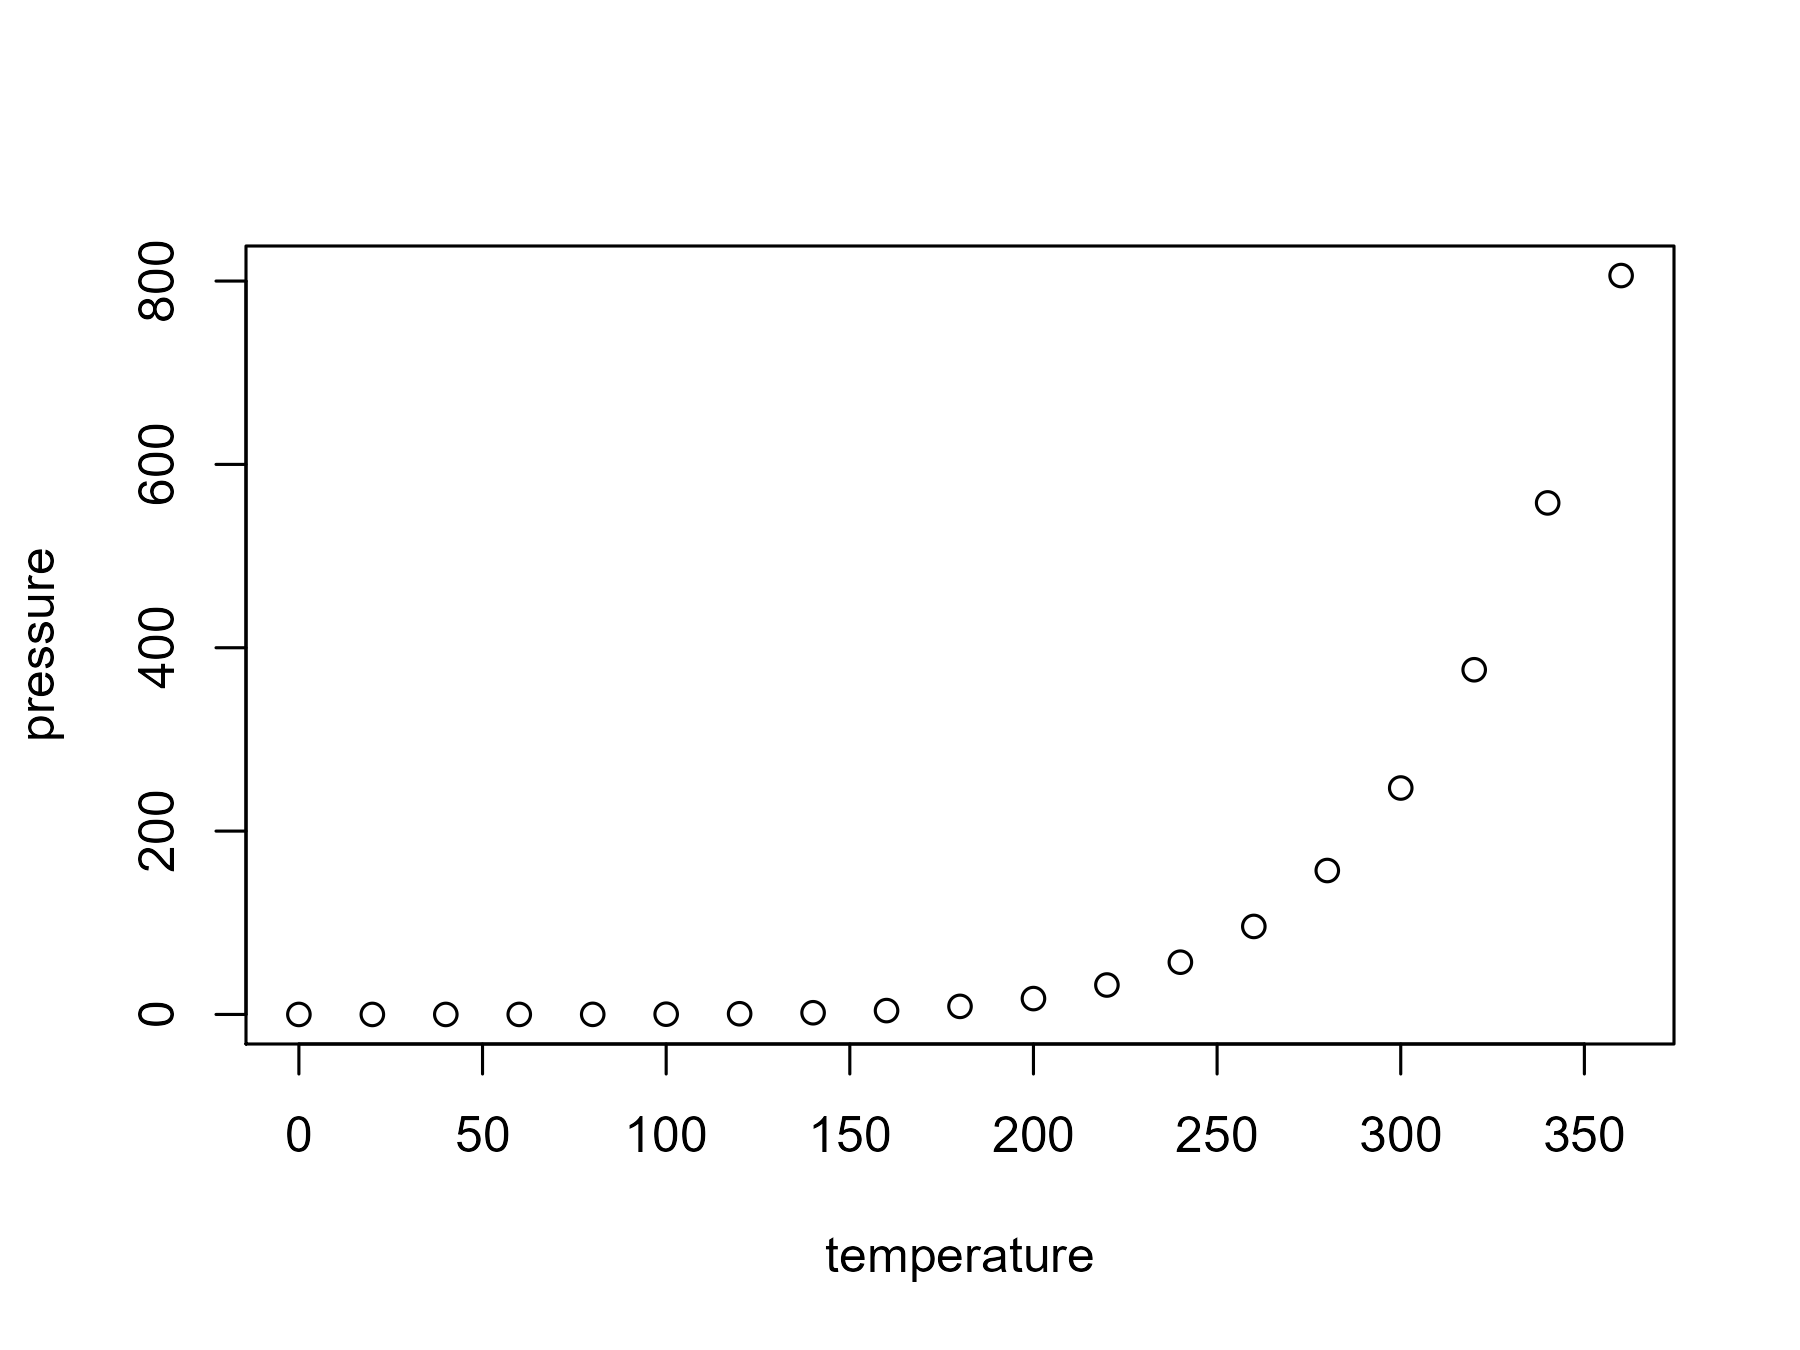
\includegraphics{C:/Data-Analysis-Projects/twriTemplates/tests/testthat/rendered/twri-pdf-test_files/figure-latex/pressure-1} \caption{pressure dataset}\label{fig:pressure}
\end{figure}

\newpage
\blandscape

\hypertarget{landscape-section}{%
\section{Landscape Section}\label{landscape-section}}

\begin{figure}

{\centering 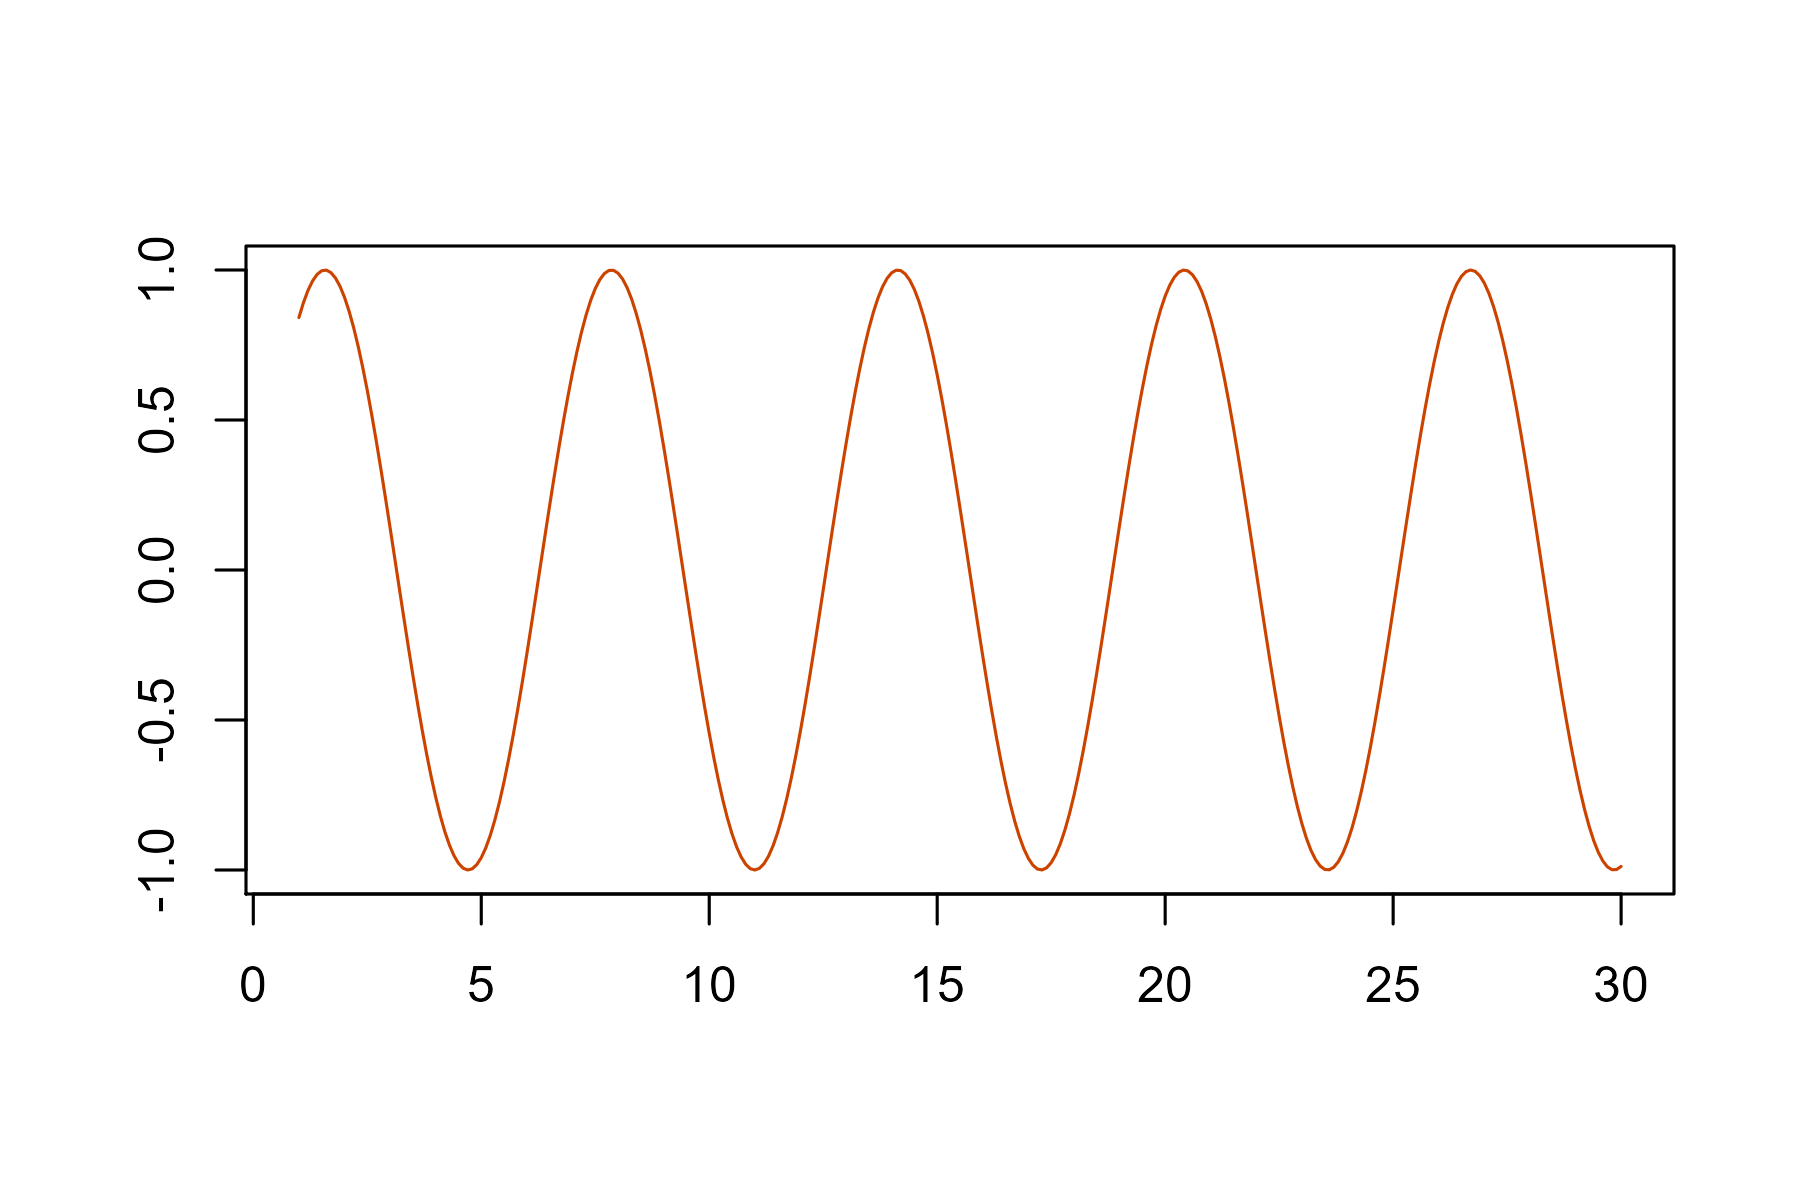
\includegraphics{C:/Data-Analysis-Projects/twriTemplates/tests/testthat/rendered/twri-pdf-test_files/figure-latex/unnamed-chunk-1-1} 

}

\caption{sin function}\label{fig:unnamed-chunk-1}
\end{figure}

\elandscape
\newpage

\hypertarget{math}{%
\section{Math}\label{math}}

Wrap variables or math in a single \texttt{\$} to show math inline. For example, \(\varepsilon \sim \mathrm{N}(0,1)\). Standalone equations are wrapped with \texttt{\$\$}.

\[
\left(\prod_{i=1}^{n}y_i\right)^{\frac{1}{n}} = 
\exp\left[\frac{1}{n}\sum_{i=1}^n\log{y_i}\right], 
\quad \textrm{when} \quad y_1, y_2, ..., y_n > 0
\]

If the equations need to be numbered and cross-referenced the format as:

\begin{Shaded}
\begin{Highlighting}[]
\KeywordTok{\textbackslash{}begin}\NormalTok{\{}\ExtensionTok{equation}\NormalTok{\}}
\SpecialCharTok{\textbackslash{}left}\SpecialStringTok{(}\SpecialCharTok{\textbackslash{}prod}\SpecialStringTok{\_\{i=1\}\^{}\{n\}y\_i}\SpecialCharTok{\textbackslash{}right}\SpecialStringTok{)\^{}\{}\SpecialCharTok{\textbackslash{}frac}\SpecialStringTok{\{1\}\{n\}\} = }
\SpecialCharTok{\textbackslash{}exp\textbackslash{}left}\SpecialStringTok{[}\SpecialCharTok{\textbackslash{}frac}\SpecialStringTok{\{1\}\{n\}}\SpecialCharTok{\textbackslash{}sum}\SpecialStringTok{\_\{i=1\}\^{}n}\SpecialCharTok{\textbackslash{}log}\SpecialStringTok{\{y\_i\}}\SpecialCharTok{\textbackslash{}right}\SpecialStringTok{], }
\SpecialCharTok{\textbackslash{}quad}\SpecialStringTok{ }\SpecialCharTok{\textbackslash{}textrm}\NormalTok{\{when\}}\SpecialStringTok{ }\SpecialCharTok{\textbackslash{}quad}\SpecialStringTok{ y\_1, y\_2, ..., y\_n \textgreater{} 0}
\SpecialStringTok{(}\SpecialCharTok{\textbackslash{}\#}\SpecialStringTok{eq:gmean)}
\KeywordTok{\textbackslash{}end}\NormalTok{\{}\ExtensionTok{equation}\NormalTok{\}}
\end{Highlighting}
\end{Shaded}

Which renders as (Equation \eqref{eq:gmean}):

\begin{equation}
\left(\prod_{i=1}^{n}y_i\right)^{\frac{1}{n}} = 
\exp\left[\frac{1}{n}\sum_{i=1}^n\log{y_i}\right], 
\quad \textrm{when} \quad y_1, y_2, ..., y_n > 0
\label{eq:gmean}
\end{equation}

\hypertarget{references}{%
\section{References}\label{references}}

In-text references and bibliography generation are handled automatically. It relies on creating a bibtex \texttt{.bib} file with your references. Software such as Zotero, Mendely, and even Google Scholar can generate the bibtex entries for you. The entries are stored in the \texttt{bibliography.bib} file inside the same directory as this \texttt{.Rmd} file. There is an example file in the same directory as this \texttt{.Rmd} file that you can update with your bibliographic entries. To make a in-text citation, use the following syntax, \texttt{{[}@helsel\_statistical\_2002{]}} to generate the reference at the end of this sentence (Helsel and Hirsch 2002). Use a semicolon to include multiple references \texttt{{[}@helsel\_statistical\_2002;\ @hirsch2010weighted{]}} (Helsel and Hirsch 2002; Hirsch et al. 2010). Or we might use \texttt{@helsel\_statistical\_2002} without brackets to indicate Helsel and Hirsch (2002) provide a fundamental overview of water quality statistics. The bibliography will populate automatically.

\hypertarget{styling-and-fonts}{%
\section{Styling and fonts}\label{styling-and-fonts}}

This template uses Minion Pro for body fonts and Open Sans for headings following TWRI brand guidance and AgriLife brand guidance. I can't bundle Minion Pro in this package because of licensing, but you can download and install both fonts from AgriLife (\url{https://agrilife.tamu.edu/wp-content/uploads/2021/03/AgriFonts.zip}). I recommend downloading and installing the fonts before knitting your documents.

\hypertarget{bibliography}{%
\section*{Bibliography}\label{bibliography}}
\addcontentsline{toc}{section}{Bibliography}

\hypertarget{refs}{}
\begin{CSLReferences}{0}{0}
\leavevmode\hypertarget{ref-helsel_statistical_2002}{}%
Helsel D, Hirsch R. 2002. Statistical methods in water resources. U.S. Geological Survey (Techniques of water-resources investigations of the {United States Geologic Survey}). \url{http://water.usgs.gov/pubs/twri/twri4a3/}.

\leavevmode\hypertarget{ref-hirsch2010weighted}{}%
Hirsch RM, Moyer DL, Archfield SA. 2010. Weighted regressions on time, discharge, and season {(WRTDS)}, with an application to {Chesapeake} {Bay} river inputs. JAWRA Journal of the American Water Resources Association. 46(5):857--880. doi:\href{https://doi.org/10.1111/j.1752-1688.2010.00482.x}{10.1111/j.1752-1688.2010.00482.x}.

\end{CSLReferences}

\newpage

\hypertarget{appendix-a}{%
\section*{Appendix A}\label{appendix-a}}
\addcontentsline{toc}{section}{Appendix A}

You can add more info, tables, and figures here.

\end{document}
